\section{Техническое задание}
\subsection{Основание для разработки}

Основанием для разработки является задание на выпускную квалификационную работу бакалавра "<Бизнес-проект \textquotedbl Кроссплатформенная программная система поиска попутчиков для автомобильных поездок\textquotedbl. Разработка серверной части">.

\subsection{Назначение разработки}

Функциональное назначение разрабатываемой кроссплатформенной программной системы заключается в предоставлении пользователям функциональных возможностей для поиска и создания автомобильных поездок.

Предполагается, что разрабатываемая программная система будет использоваться широким кругом лиц, заинтересованных в соместных поезках по России.

\subsection{Требования к программной системе}
\subsubsection{Требования к данным программной системы}

Входными данными для серверной части программной системы являются:

\begin{itemize}
	\item данные пользователя при регистрации;
	\item запрос регистрацию пользователя как водителя;
	\item данные пользователя для входа в систему;
	\item запрос на добаление автомобиля;
	\item запрос на удаление автомобиля;
	\item запрос на изменение пользовательских данных;
	\item запрос на изменение данных об автомобилях;
	\item фото профиля;
	\item данные о планируемой поездке;
	\item запрос на удаление поездки;
	\item запрос на поиск активных поездок;
	\item запрос на добаление попутчика к поездке;
	\item запрос на удаление пользователя из поездки;
	\item запрос на создание чата;
	\item запрос на просмотр активных чатов;
	\item текст сообщения;
	\item запрос на просмотр сообщений по чату;
	\item текст комментария;
	\item запрос просмотр комментариев по профилю пользователя.
\end{itemize} 

Выходными данными для серверной части программной системы являются:

\begin{itemize}
	\item данные профиля для попутчика;
	\item данные профиля для водителя;
	\item информация об автомобилях;
	\item данные об активных поездках для попутчика;
	\item данные об активнх поездках для водителя;
	\item информацию об архивных поездках;
	\item фото профиля;
	\item список активных чатов;
	\item список сообщений по чату;
	\item список доступных поездок по заданным критериям поиска;
	\item отзывы и рейтинг пользователя;
\end{itemize}

\subsubsection{Функциональные требования к программной системе}

В разрабатываемой программной системе для пользовательской части должны быть реализованы следующие функции:

\begin{enumerate}
	\item Регистрация пользователя под аккаунтом попутчика. 
	\item Регистрация пользователя под аккаунтом водителя.
	\item Получение информации о пользовательских данных.
	\item Редактирование сведений о пользователе.
	\item Получение информации об автомобилях водителя.
	\item Добавление автомобиля если пользователь является водителем.
	\item Редактирование сведений об автомобиле.
	\item Удаление автомобиля.
	\item Отправка фотографии на пользовательскую часть программной системы.
	\item Смена фотографии пользователя.
	\item Получение информации о пользовательских поездках.
	\item Создание поездки под аккаунтом водителя.
	\item Удаление поездки под аккаунтом водителя.
	\item Добавление в архив не актуальных поездок.
	\item Поиск поездки по заданным критериям.
	\item Бронирование поездки.
	\item Отмена брони.
	\item Создание чата с водителем под аккаунтном попутчика.
	\item Получение информации о пользовательских чатах.
	\item Получение сообщений по указанному чату.
	\item Добавление нового сообщения.
	\item Получение информации об отзывах и оценках.
	\item Добавление отзыва и оценки.
	\item Удаление отзыва.
\end{enumerate}

На рисунках 2.1-2.3 представлены функциональные требования к системе в виде диаграммы прецедентов нотации UML.

\begin{figure}[H]
	\centering
	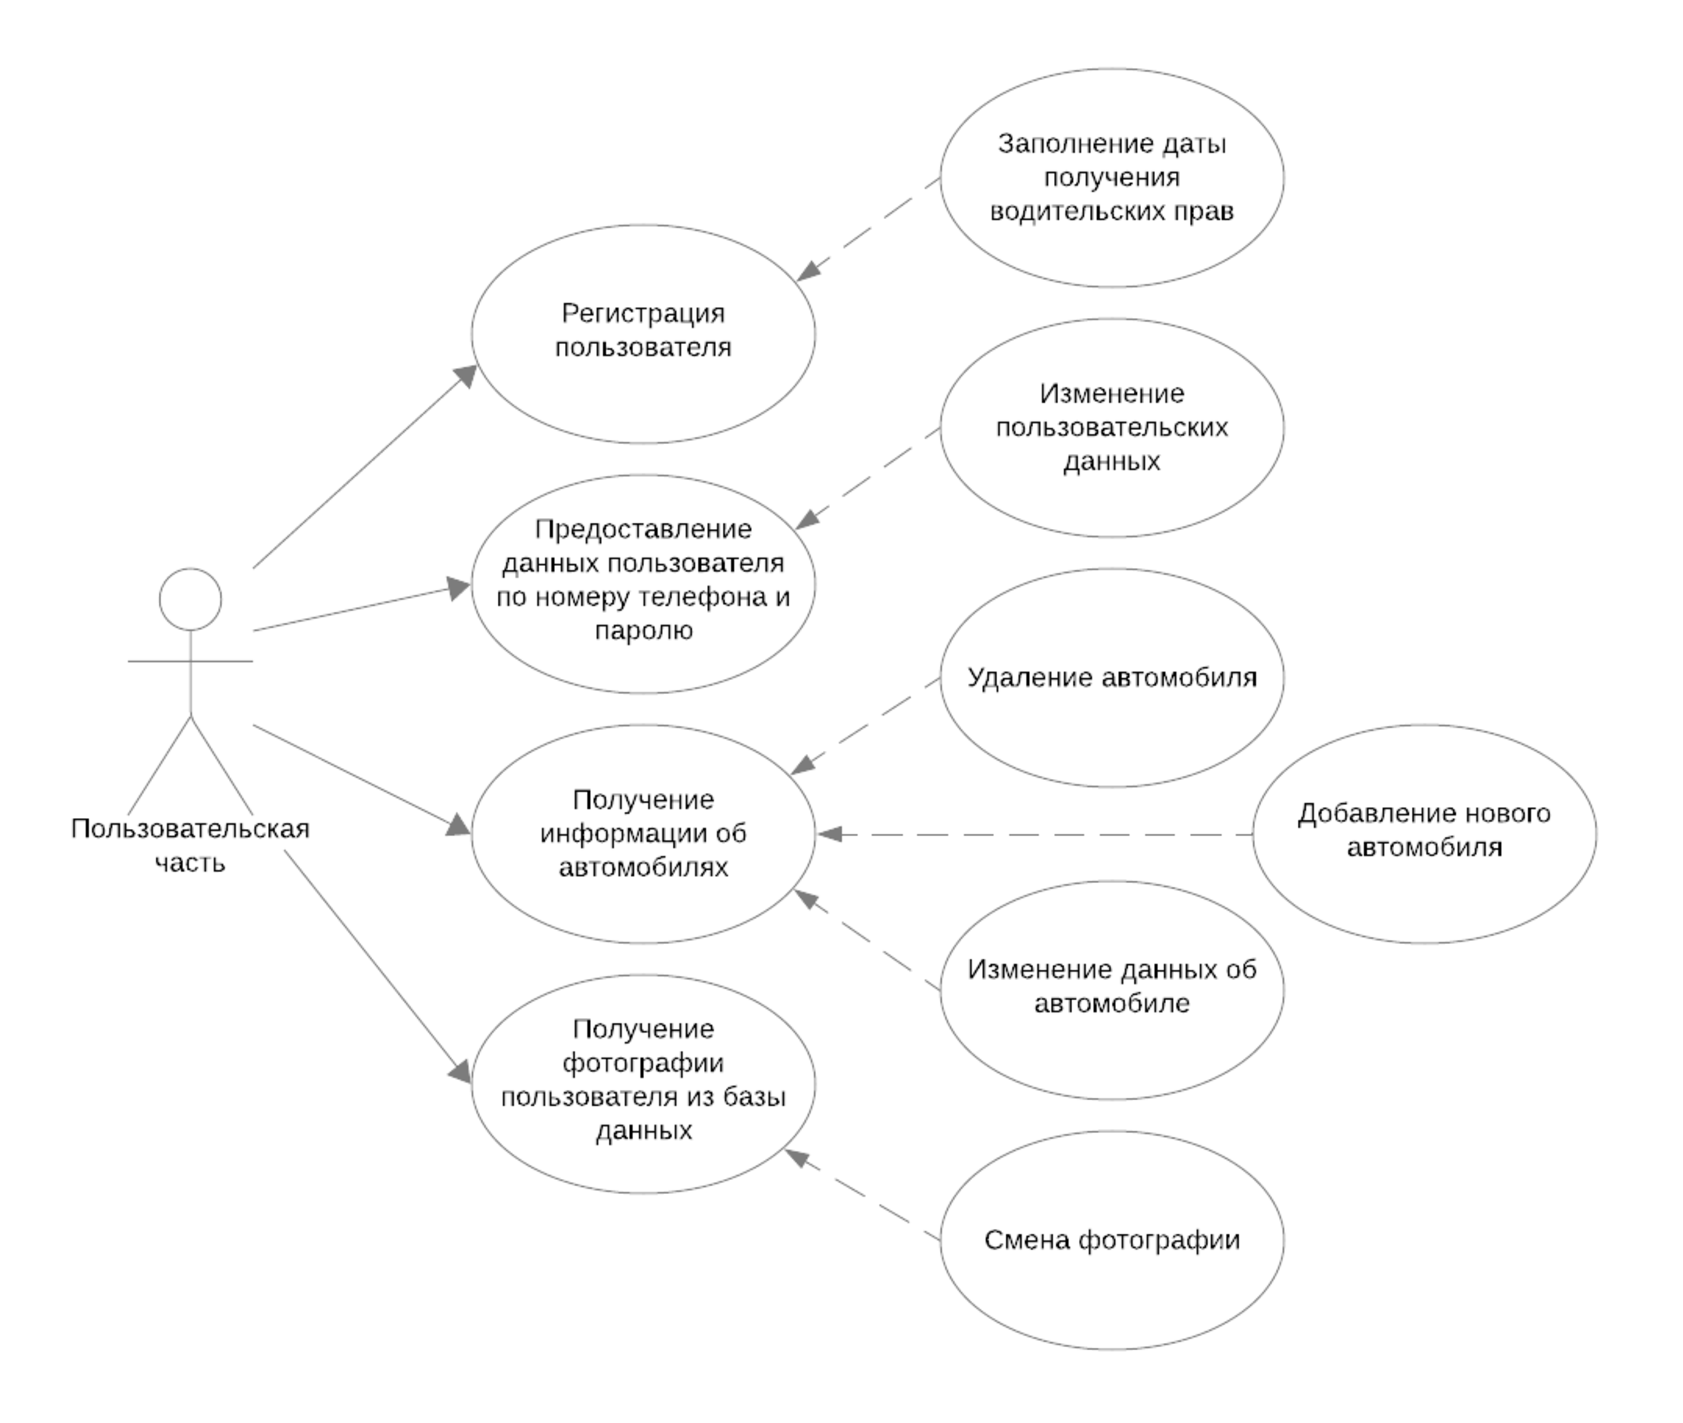
\includegraphics[width=0.7\linewidth]{images/Precedent1}
	\caption{Диаграмма вариантов использования, часть 1}
	\label{fig:precedent1}
\end{figure}

\begin{figure}[H]
	\centering
	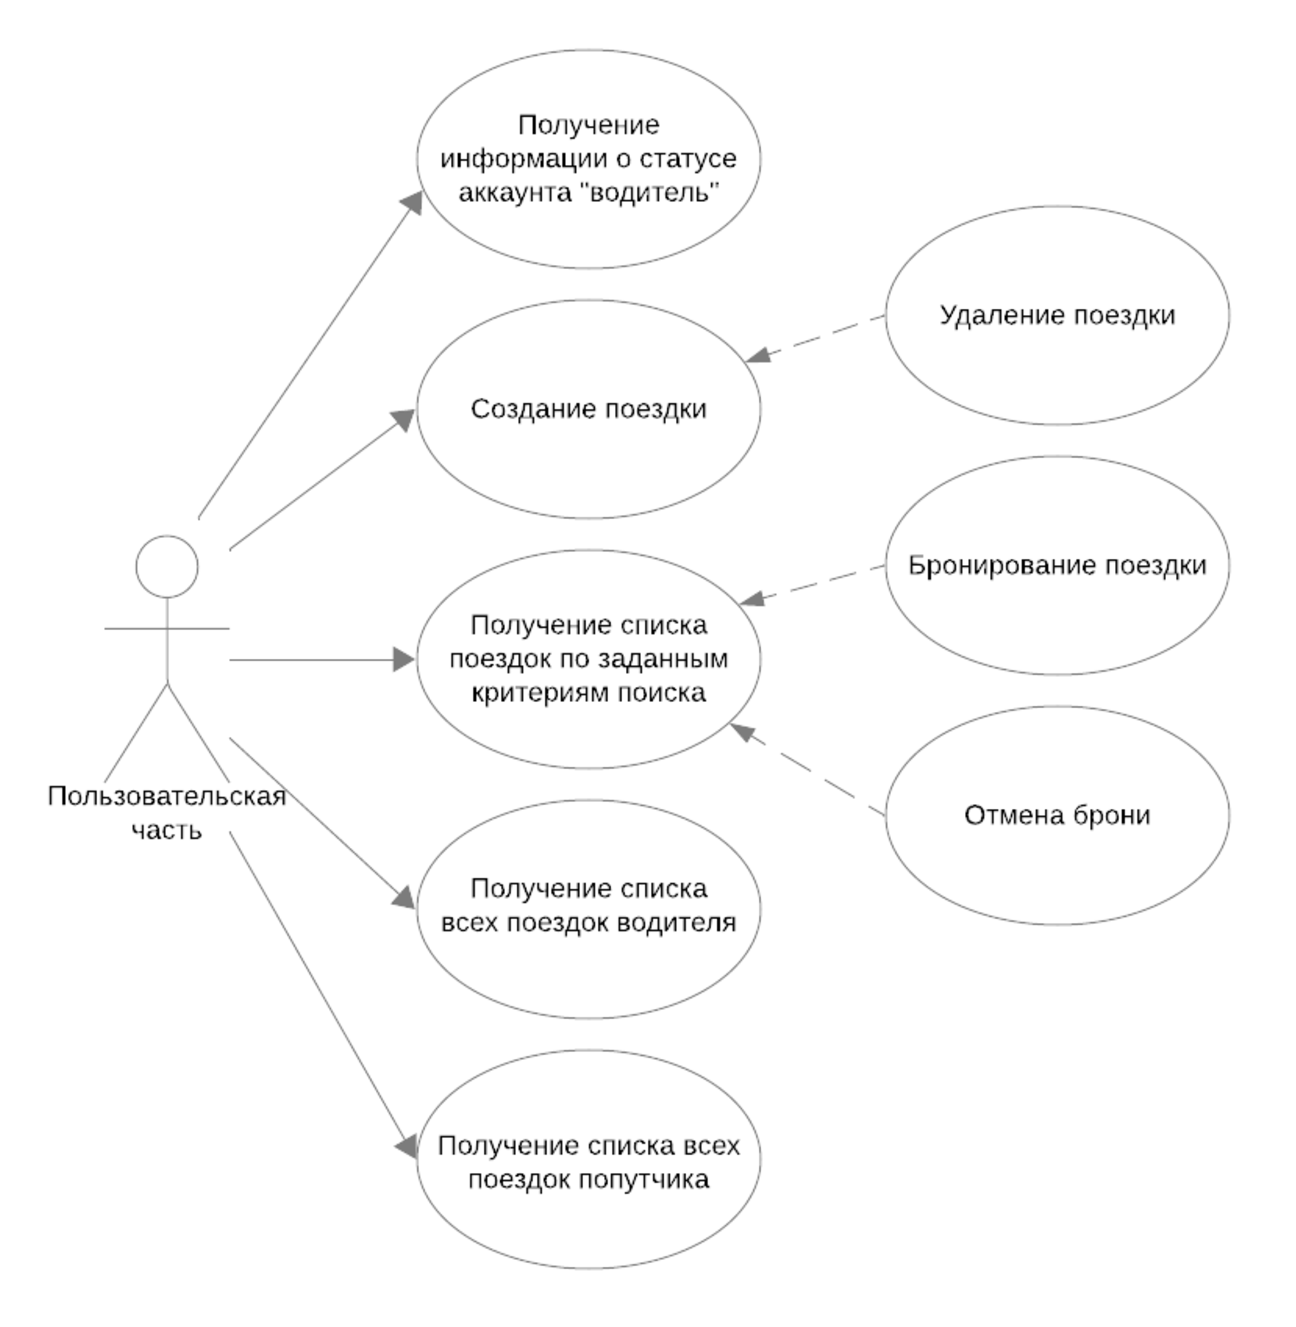
\includegraphics[width=0.7\linewidth]{images/Precedent2}
	\caption{Диаграмма вариантов использования, чать 2}
	\label{fig:precedent2}
\end{figure}

\begin{figure}[H]
	\centering
	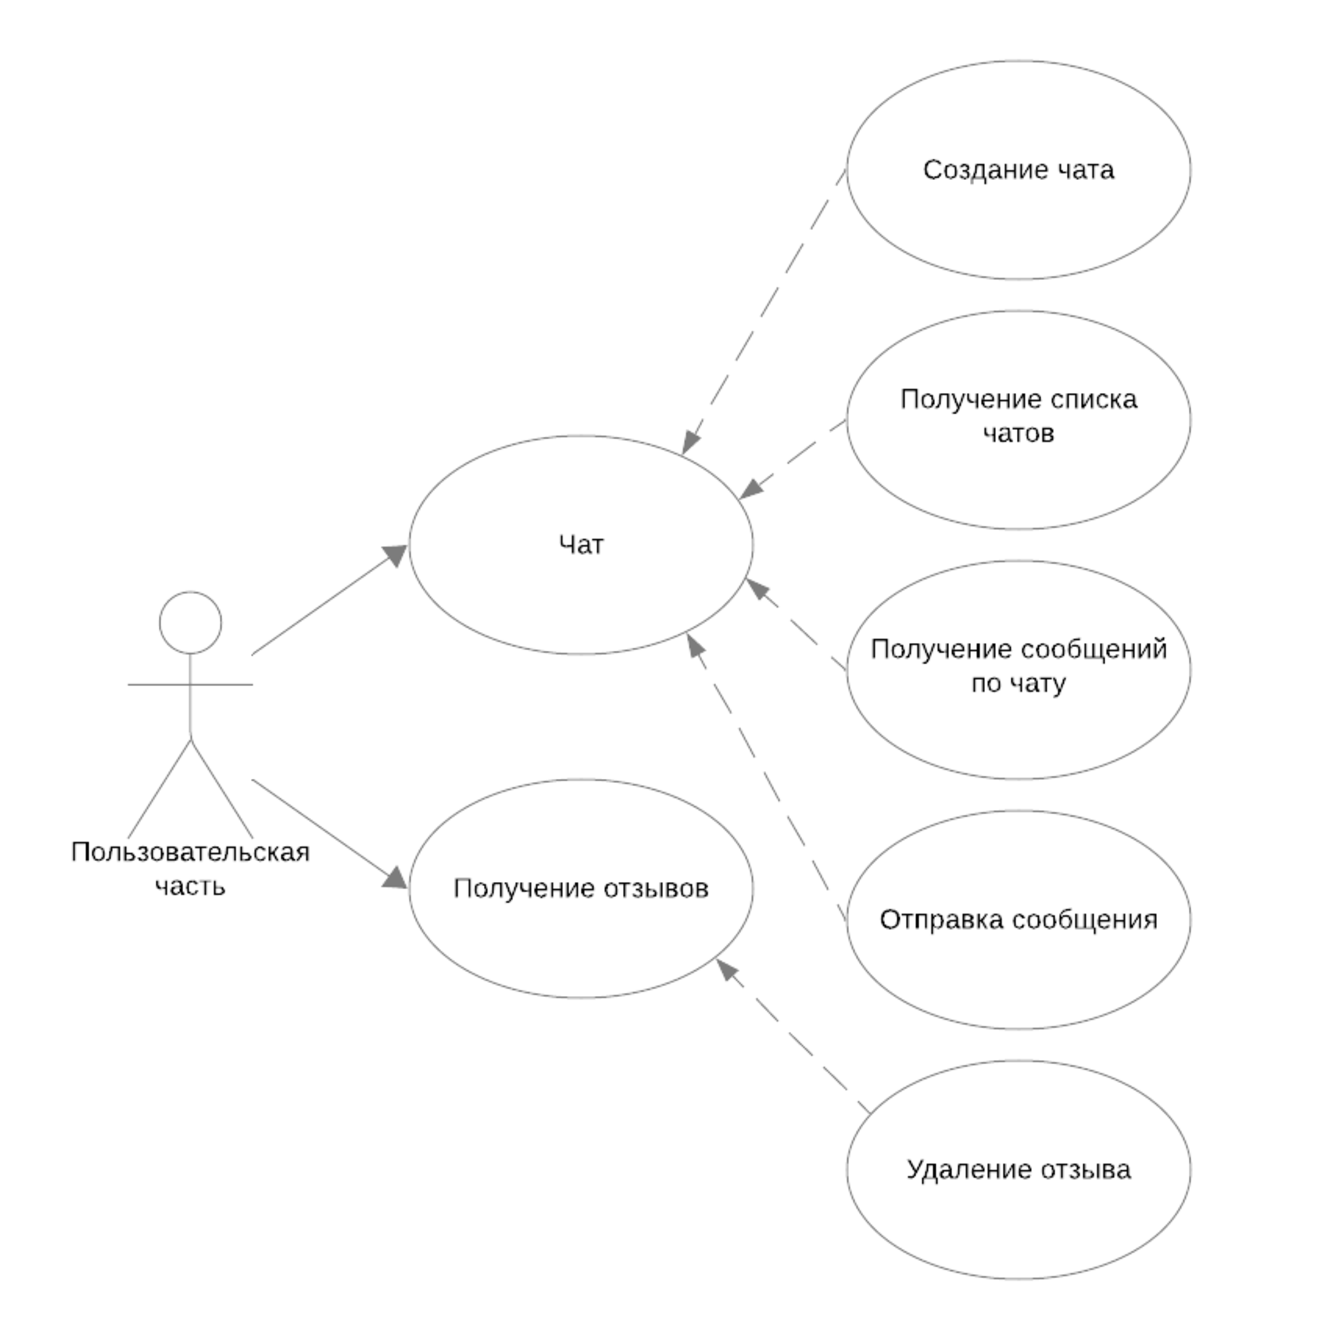
\includegraphics[width=0.7\linewidth]{images/Precedent3}
	\caption{Диаграмма вариантов использования, часть 3}
	\label{fig:precedent3}
\end{figure}

\paragraph{Вариант использования «Регистрация пользователя»}
Заинтересованные лица и их требования: пользователи программной системы, которые хотят зарегистрировать аккаунт, с целью получения возможности использовать функционал приложения для подбора попутчиков. Предусловие: на пользовательском устройстве открыто приложение AutoStop. Постусловие: пользователь регистрирует аккаунт как попутчик.
Основной успешный сценарий:

\begin{enumerate}
	\item Со стороны пользовательской части на сервер отправеляется URI запрос с пользовательскими данными в формате json файла.
	\item Сервер отслеживает запрос, проверяя возможность регистрации под переданным номером телефона.
	\item Сервер запускает скрипт на добавление пользователя в базу данных.
	\item Сервер отправляет на frontend статус OK.
\end{enumerate}

\paragraph{Вариант использования «Регистрация водителя»}
Заинтересованные лица и их требования: пользователи программной системы, которые хотят расширить возможности своей учетной записи, с целью создания поездок в используемом приложении. Предусловие: пользователь уже осуществил базовую регистрацию аккаунта. Постусловие: пользователь регистрирует аккаунт как водитель.
Основной успешный сценарий:

\begin{enumerate}
	\item Со стороны пользовательской части на сервер отправеляется URI запрос с номером телефона пользователя и датой получения водительского удостоверения.
	\item Сервер отслеживает запрос, и дополняет информацию по аккаунту пользователя.
	\item Сервер отправляет на frontend статус OK.
\end{enumerate}

\paragraph{Вариант использования «Авторизация»}
Заинтересованные лица и их требования: пользователи программной системы, которые хотят войти в систему подбора попутчиков для автомобильных поездок под своей учетной записью. Предусловие: пользователь прошел регистрацию и имеет аккаунт. Постусловие: пользователь входит в систему.
Основной успешный сценарий:

\begin{enumerate}
	\item Со стороны пользовательской части на сервер отправеляется URI запрос с номером телефона пользователя и паролем в формате json файла.
	\item Сервер отслеживает запрос, и находит пользователя по переданным данным.
	\item Сервер отправляет на frontend json файл с пользовательскими данными.
\end{enumerate}

\paragraph{Вариант использования «Изменение пользовательских данных»}
Заинтересованные лица и их требования: пользователи программной системы, которые хотят изменить личные данные в системе подбора попутчиков для автомобильных поездок. Предусловие: пользователь осуществил вход под своей учетной записью. Постусловие: пользователь изменяет данные аккаунта.
Основной успешный сценарий:

\begin{enumerate}
	\item Со стороны пользовательской части на сервер отправеляется URI запрос с номером телефона пользователя и измененными данными в формате json файла.
	\item Сервер отслеживает запрос, и находит пользователя по переданным данным.
	\item Сервер запускает скрипт на изменение в БД.
	\item Сервер отправляет на frontend статус OK.
\end{enumerate}

\paragraph{Вариант использования «Получение информации об автомобилях»}
Заинтересованные лица и их требования: пользователи программной системы, которые хотят получить список всех автомобилей, доступных под используемым профилем. Предусловие: пользователь осуществил вход под своей учетной записью и является водителем в системе. Постусловие: пользователь получает список машин.
Основной успешный сценарий:

\begin{enumerate}
	\item Со стороны пользовательской части на сервер отправеляется URI запрос с номером телефона пользователя.
	\item Сервер отслеживает запрос, и находит все автомобили зарегистрированные на данного пользователя.
	\item Сервер отправляет на frontend список всех найденых машин.
\end{enumerate}

\paragraph{Вариант использования «Добавление нового автомобиля»}
Заинтересованные лица и их требования: пользователи программной системы, которые хотят добавить автомобиль, для дальнейшего использования в поездках. Предусловие: пользователь осуществил вход под своей учетной записью и является водителем в системе. Постусловие: пользователь добавляет автомобиль в свой профиль.
Основной успешный сценарий:

\begin{enumerate}
	\item Со стороны пользовательской части на сервер отправеляется URI запрос с номером телефона пользователя и данными об автомобиле в формате json файла.
	\item Сервер отслеживает запрос, и добавляет сведения об автомобиле указанному пользователю.
	\item Сервер отправляет на frontend сообщение со статусом OK.
\end{enumerate}

\paragraph{Вариант использования «Изменение данных об автомобиле»}
Заинтересованные лица и их требования: пользователи программной системы, которые изменить указанные данные о машине в профиле. Предусловие: пользователь осуществил вход под своей учетной записью и является водителем в системе. У пользователя есть хотя бы 1 автомобиль в профиле. Постусловие: пользователь изменяеь данные о машине.
Основной успешный сценарий:

\begin{enumerate}
	\item Со стороны пользовательской части на сервер отправеляется URI запрос с ГРЗ автомобиля и обновленными данными в формате json файла.
	\item Сервер отслеживает запрос, и обновляет данные, на новые.
	\item Сервер отправляет на frontend сообщение со статусом OK.
\end{enumerate}

\paragraph{Вариант использования «Удаление автомобиля»}
Заинтересованные лица и их требования: пользователи программной системы, которые хотят удалить существующий автомобиль из профиля. Предусловие: пользователь осуществил вход под своей учетной записью и является водителем в системе. У пользователя есть хотя бы 1 автомобиль в профиле. Постусловие: пользователь удаляет данные о машине.
Основной успешный сценарий:

\begin{enumerate}
	\item Со стороны пользовательской части на сервер отправеляется URI запрос с ГРЗ автомобиля который необходимо удалить.
	\item Сервер отслеживает запрос, и находит указанную машину.
	\item Сервер запускает скрипт на удаление автомобиля из БД.
	\item Сервер отправляет на frontend сообщение со статусом OK.
\end{enumerate}

\paragraph{Вариант использования «Получение фото профиля»}
Заинтересованные лица и их требования: пользователи программной системы, которые осуществляют вход под своей учетной записью. Предусловие: пользователь прошел базовую регистрацию и имеет аккаунт в системе. Постусловие: пользователь получает фотографию своего профиля.
Основной успешный сценарий:

\begin{enumerate}
	\item Со стороны пользовательской части на сервер отправеляется URI запрос с номером телефона пользователя.
	\item Сервер отслеживает запрос, и находит фото профиля в базе данных.
	\item Сервер отправляет на frontend изображение.
\end{enumerate}

\paragraph{Вариант использования «Смена фото профиля»}
Заинтересованные лица и их требования: пользователи программной системы, которые хотят заменить фотографию профиля на новую. Предусловие: пользователь прошел базовую регистрацию и имеет аккаунт в системе. Постусловие: пользователь изменяет фотографию своего профиля.
Основной успешный сценарий:

\begin{enumerate}
	\item Со стороны пользовательской части на сервер отправеляется URI запрос с номером телефона пользователя и фографией в формате json файла.
	\item Сервер отслеживает запрос, и находит пользователя с указанным номером телефона.
	\item Сервер запускает скрипт на изменение фотографии в БД.
	\item Сервер отправляет на frontend сообщение со статусом OK.
\end{enumerate}

\paragraph{Вариант использования «Получение информации о статусе аккаунта}
Заинтересованные лица и их требования: пользователи программной системы, которые хотят создать новую поездку в системе. Предусловие:  пользователь вошел под своим аккунтом в приложение. Постусловие: пользователь получает возможность создать поездку в системе.
Основной успешный сценарий:

\begin{enumerate}
	\item Со стороны пользовательской части на сервер отправеляется URI запрос с номером телефона пользователя.
	\item Сервер отслеживает запрос, и находит запись с датой получения водительского удостоверения.
	\item Сервер отправляет на frontend json файл с датой получения прав.
\end{enumerate}

\paragraph{Вариант использования «Создание поездки»}
Заинтересованные лица и их требования: пользователи программной системы, которые хотят создать новую поездку в системе. Предусловие:  пользователь вошел под своим аккунтом в приложение и прошел проверку на наличие водительского удостоверения. Постусловие: пользователь создает поезку в системе для подбора попутчиков.
Основной успешный сценарий:

\begin{enumerate}
	\item Со стороны пользовательской части на сервер отправеляется URI запрос с данными о поездке, которую необходимо создать, в формате json файла.
	\item Сервер отслеживает запрос, и добавляет данные о поездке в БД.
	\item Сервер отправляет на frontend сообщение со статусом  OK.
\end{enumerate}

\paragraph{Вариант использования «Удаление поездки»}
Заинтересованные лица и их требования: пользователи программной системы, у которых есть необходимость у далении существующей поездки. Предусловие:  пользователь вошел под своим аккунтом в приложение. В системе есть хотя бы одна поездка созданная до данным профилем. Постусловие: пользователь удаляет поезку в системе для подбора попутчиков.
Основной успешный сценарий:

\begin{enumerate}
	\item Со стороны пользовательской части на сервер отправеляется URI запрос уникальным идентификатором удаляемой поездки.
	\item Сервер отслеживает запрос, и удаляет поездку из системы.
	\item Сервер отправляет на frontend сообщение со статусом  OK.
\end{enumerate}

\paragraph{Вариант использования «Получение списка поездок по заданным критериям поиска»}
Заинтересованные лица и их требования: пользователи программной системы, у которых есть необходимость в поиске подходящей поездки. Предусловие:  пользователь вошел под своим аккунтом в приложение. Постусловие: попутчик получает список поездок по заданным условиям поиска.
Основной успешный сценарий:

\begin{enumerate}
	\item Со стороны пользовательской части на сервер отправеляется URI запрос с данными, на основе которых необходимо осуществить выборку из существующих поездок в системе.
	\item Сервер отслеживает запрос, и находит все поездки, удовлетворящие условиям поиска.
	\item Сервер отправляет на frontend список всех найденых поездок в формате json файла.
\end{enumerate}

\paragraph{Вариант использования «Бронирование поездки»}
Заинтересованные лица и их требования: пользователи программной системы, целью которых является бронирование поездки в системе для подбора попутчиков. Предусловие:  пользователь вошел под своим аккунтом в приложение. В системе имеются активные поездки. Постусловие: попутчик бронирует поездку.
Основной успешный сценарий:

\begin{enumerate}
	\item Со стороны пользовательской части на сервер отправеляется URI запрос с пользовательскими данные и информацией о бронируемой поездке.
	\item Сервер отслеживает запрос, и записывает пользователя в поездку.
	\item Сервер отправляет на frontend ответ со статусом OK.
\end{enumerate}

\paragraph{Вариант использования «Отмена брони»}
Заинтересованные лица и их требования: пользователи программной системы, которые хотят отменить бронирование поездки. Предусловие:  пользователь вошел под своим аккунтом в приложение. У пользователя есть бронь. Постусловие: попутчик отменяет бронь.
Основной успешный сценарий:

\begin{enumerate}
	\item Со стороны пользовательской части на сервер отправеляется URI запрос с пользовательскими данные и информацией о бронируемой поездке.
	\item Сервер отслеживает запрос, и удаляет из базы данных информацию о брони.
	\item Сервер отправляет на frontend ответ со статусом OK.
\end{enumerate}

\paragraph{Вариант использования «Получения списка всех поездок для водителя»}
Заинтересованные лица и их требования: пользователи программной системы, получить список всех созданных поездок данным водителем. Предусловие:  пользователь вошел под своим аккунтом в приложение. У пользователя есть хотя бы одна созданная поездка. Постусловие: водитель получает список всех созданных поездок.
Основной успешный сценарий:

\begin{enumerate}
	\item Со стороны пользовательской части на сервер отправеляется URI запрос с номером телефона водителя.
	\item Сервер отслеживает запрос, и находит пользовательские поездки.
	\item Сервер отправляет на frontend список всех созданных поездок со статусом "<водитель"> в формате json файла.
\end{enumerate}

\paragraph{Вариант использования «Получения списка всех поездок для водителя»}
Заинтересованные лица и их требования: пользователи программной системы, получить список всех созданных поездок данным водителем. Предусловие:  пользователь вошел под своим аккунтом в приложение. У пользователя есть хотя бы одна созданная поездка. Постусловие: водитель получает список всех созданных поездок.
Основной успешный сценарий:

\begin{enumerate}
	\item Со стороны пользовательской части на сервер отправеляется URI запрос с номером телефона водителя.
	\item Сервер отслеживает запрос, и находит пользовательские поездки.
	\item Сервер отправляет на frontend список всех созданных поездок со статусом "<водитель"> в формате json файла.
\end{enumerate}

\paragraph{Вариант использования «Получения списка всех поездок для попутчика»}
Заинтересованные лица и их требования: пользователи программной системы, получить список всех забронированных поездок. Предусловие:  пользователь вошел под своим аккунтом в приложение. У пользователя есть хотя бы одна забронированная поездка. Постусловие: попутчик получает список всех созданных поездок.
Основной успешный сценарий:

\begin{enumerate}
	\item Со стороны пользовательской части на сервер отправеляется URI запрос с номером телефона попутчика.
	\item Сервер отслеживает запрос, и находит пользовательские поездки.
	\item Сервер отправляет на frontend список всех забронированных поездок в формате json файла.
\end{enumerate}

\paragraph{Вариант использования «Создание чата»}
Заинтересованные лица и их требования: пользователи программной системы, которые хотят свзяаться с водителем для обсуждения планов поездки. Предусловие:  пользователь вошел под своим аккунтом в приложение и осуществил поиск поездок. Постусловие: попутчик создает чат с водителем.
Основной успешный сценарий:

\begin{enumerate}
	\item Со стороны пользовательской части на сервер отправеляется URI запрос с номеромами телефона попутчика и водителя.
	\item Сервер отслеживает запрос, и проверяет наличие чата.
	\item Сервер создает новый чат.
	\item Сервер отправляет на frontend информацию о новом созданном чате в формате json файла.
\end{enumerate}

\paragraph{Вариант использования «Получение списка чатов»}
Заинтересованные лица и их требования: пользователи программной системы, которые хотят получить полную информацю по имеющимся чатам. Предусловие:  пользователь вошел под своим аккунтом в приложение и имеет хотя бы 1 чат. Постусловие: пользователь получает полный список чатов.
Основной успешный сценарий:

\begin{enumerate}
	\item Со стороны пользовательской части на сервер отправеляется URI запрос с номеромами телефона пользователя.
	\item Сервер отслеживает запрос, и находит информацю по чатам.
	\item Сервер отправляет на frontend список всех чатов в формате json файла.
\end{enumerate}

\paragraph{Вариант использования «Получение сообщений по чату»}
Заинтересованные лица и их требования: пользователи программной системы, которые хотят получить все сообщения по выбранному чату. Предусловие:  пользователь вошел под своим аккунтом в приложение и имеет хотя бы 1 чат с сообщениями. Постусловие: пользователь получает полный список сообщений.
Основной успешный сценарий:

\begin{enumerate}
	\item Со стороны пользовательской части на сервер отправеляется URI запрос с уникальным идентификатором чата.
	\item Сервер отслеживает запрос, и находит сообщения по указанному чату.
	\item Сервер отправляет на frontend список всех сообщений в формате json файла.
\end{enumerate}

\paragraph{Вариант использования «Отправка сообщения»}
Заинтересованные лица и их требования: пользователи программной системы, которые хотят установисть связь с собеседником через отправку сообщений. Предусловие:  пользователь вошел под своим аккунтом в приложение и имеет хотя бы 1 чат. Постусловие: пользователь отправляет сообщение собеседнику.
Основной успешный сценарий:

\begin{enumerate}
	\item Со стороны пользовательской части на сервер отправеляется URI запрос с уникальным идентификатором чата и текстом сообщения в формате json файла.
	\item Сервер отслеживает запрос, и добавляет сообщение в БД.
	\item Сервер отправляет на frontend ответ со статусом OK.
\end{enumerate}

\paragraph{Вариант использования «Получение отзывов»}
Заинтересованные лица и их требования: пользователи программной системы, которые хотят просмотреть список всех отзывов по профилю. Предусловие:  пользователь имеет хотя бы 1 отзыв. Постусловие: пользователь получает список всех отзывов.
Основной успешный сценарий:

\begin{enumerate}
	\item Со стороны пользовательской части на сервер отправеляется URI запрос с номером телефона пользователя.
	\item Сервер отслеживает запрос, и производит поик всех отзывов.
	\item Сервер отправляет на frontend список всех отзывов.
\end{enumerate}

\paragraph{Вариант использования «Удаление отзыва»}
Заинтересованные лица и их требования: пользователи программной системы, которые хотят удалить оставленный отзыв. Предусловие:  пользователь имеет хотя бы 1 отзыв. Постусловие: пользователь удаляет свой отзывов.
Основной успешный сценарий:

\begin{enumerate}
	\item Со стороны пользовательской части на сервер отправеляется URI запрос с уникальным идентификатором отзыва.
	\item Сервер отслеживает запрос, и производит удаление отзыва.
	\item Сервер отправляет на frontend ответ со статусом OK.
\end{enumerate}

\subsubsection{Нефункциональные требования к программной системе}
\paragraph{Требования к надежности}

В процессе работы серверной части программной системы могут произойти следующие аварийные ситуации:

\begin{itemize}
\item Потеря доступа к сети Интернет. Возможные причины включают проблемы с сетью, сбои маршрутизаторов или изменения в конфигурации сети.
\item Аварийное отключение электропитания. Это может произойти из-за технических проблем в дата-центре, аварий на электросетях или природных катаклизмов.
\item Сбой операционной системы сервера. Операционная система может выйти из строя по причине аппаратных или программных сбоев, ошибок обновлений или атак вредоносного ПО.
\end{itemize}

Для минимизации вероятности возникновения аварийных событий серверные компоненты программной системы должны быть размещены на выделенных серверах в дата-центрах хостинг-провайдеров. Операционная система должна получать регулярные накопительные обновления.

\paragraph{Требования к безопасности}
Для защиты системы от несанкционированного доступа каждый запрос к базе данных должен проходить через специальный набор правил. Пользователь, не имеющий доступа к определенным данным должен не
иметь возможности взаимодействовать с ними.

Для доступа к приложению пользователю необходимо пройти авторизацию в системе.

Для возможности авторизации в системе, пользователь должен пройти регистрацию.

Фунции доступные водительскому акаунту не должны быть доступны для попутчика.

\paragraph{Требования к программному обеспечению}

Для реализации серверной части программной системы должен быть использован язык высокого уровня C\#.

В качестве системы управления базой данных (СУБД) должна быть использована система Microsoft SQL Server, разработанная компанией Microsoft.

Для реализации модуля чатов и сообщений необходим асинхронный подход, для ускорения работы системы и оптимизации используемых ресурсов сервера.

За обеспечение целостности данных должнен отвечать автоматический сервис, который запускается на сервере каждые 10 минут. С целью добавления неактуальных поездок в архив. Это снизит нагрузку при поиске данных, связанных с пользовательскими поездками.

\paragraph{Требования к аппаратному обеспечению}

Для обеспечения стабильной и эффективной работы написанной программной реализации, сервер должен соответствовать следующим требованиям к аппаратному обеспечению:

Процессор (CPU)
\begin{itemize}
	\item Тип: Многоядерный процессор с поддержкой технологии многопоточности.
	\item Рекомендуемые модели: Intel Xeon серии E5 или выше, AMD EPYC или Ryzen 7 и выше.
	\item Частота: Минимум 2.4 ГГц на ядро.
	\item Количество ядер: Минимум 4 физических ядра.
\end{itemize}

Оперативная память (RAM)
\begin{itemize}
	\item Объем: Минимум 16 ГБ, рекомендуется 32 ГБ и выше в зависимости от нагрузки и количества одновременно работающих приложений.
	\item Тип: DDR4 с частотой не ниже 2400 МГц.
\end{itemize}

Накопитель (SSD/HDD)
\begin{itemize}
	\item Тип: SSD для основной системы и данных, HDD можно использовать для хранения архивов и резервных копий.
	\item Объем: Минимум 500 ГБ для SSD, рекомендуется 1 ТБ и более.
	\item Скорость чтения/записи: Не менее 500 МБ/с для SSD.
\end{itemize}

Сетевое оборудование
\begin{itemize}
	\item Сетевая карта: Гигабитная Ethernet-карта (1 Gbps).
	\item Дополнительно: Поддержка резервирования сетевых подключений для обеспечения отказоустойчивости.
\end{itemize}

Источник бесперебойного питания (ИБП)
\begin{itemize}
	\item Мощность: Достаточная для поддержания работы сервера в течение минимум 30 минут при отключении электропитания.
	\item Функции: Возможность автоматического корректного завершения работы сервера при длительном отключении питания.
\end{itemize}

Система охлаждения
\begin{itemize}
	\item Тип: Эффективная система охлаждения для поддержания стабильной температуры процессора и других компонентов.
	\item Дополнительно: Наличие нескольких вентиляторов и/или жидкостной системы охлаждения для серверов с высокими нагрузками.
\end{itemize}

Корпус и питание
\begin{itemize}
	\item Корпус: Серверный корпус форм-фактора Tower или Rack, обеспечивающий хорошую вентиляцию.
	\item Блок питания: Сертифицированный блок питания с мощностью не менее 750 Вт, с запасом мощности для дополнительного оборудования.
\end{itemize}

Дополнительные требования
\begin{itemize}
	\item Резервирование: Возможность установки резервных блоков питания и дисков для обеспечения отказоустойчивости.
	\item Мониторинг: Встроенные системы мониторинга состояния компонентов и температуры.
\end{itemize}

\subsection{Требования к оформлению документации}
Требования к стадиям разработки программ и программной документации для вычислительных машин, комплексов и систем независимо от их
назначения и области применения, этапам и содержанию работ устанавливаются ГОСТ 19.102–77.
Программная документация должна включать в себя:
\begin{itemize}
\item Анализ предметной области.
\item Техническое задание.
\item Технический проект.
\item Рабочий проект.
\end{itemize}